\documentclass{sig-alternate}
%[preprint]
% The following \documentclass options may be useful:
%
% 10pt          To set in 10-point type instead of 9-point.
% 11pt          To set in 11-point type instead of 9-point.
% authoryear    To obtain author/year citation style instead of numeric.

\makeatletter
\def\@copyrightspace{\relax}
\makeatother

\usepackage[nynorsk,british,UKenglish,USenglish,english,american]{babel}

\usepackage{graphicx}
\usepackage{tikz}
%\usepackage{gnuplot-lua-tikz}
\usepackage{color}
\usepackage{tabularx}
\usepackage{fixltx2e}
%% \usepackage{dblfloatfix}
\usepackage{varwidth} % http://ctan.org/pkg/varwidth
\usepackage{listings}
\usepackage{url}
\usepackage{balance}
\usepackage{amsmath}
\usepackage{enumitem}
\usepackage{caption}

\lstset{
%  backgroundcolor=\color{yellow!20},%
  basicstyle=\small\ttfamily,%
  numbers=left, numberstyle=\tiny%
}

\newtheorem{thm}{Problem}
\newdef{definition}{Definition}
\DeclareMathAlphabet{\mathpzc}{OT1}{pzc}{m}{it}
\newtheorem{theorem}{Theorem}[section]
\newtheorem{lemma}[theorem]{Lemma}

\usepackage{xcolor}
\usepackage{framed}
\usepackage{amssymb,amsmath}
\usepackage{ifxetex,ifluatex}
\usepackage{fancyvrb}
\usepackage{comment}

\begin{document}

\title{\Large\bf Midterm Report: Design an accelerator for Computing MRI-Q Matrix}
\subtitle{\normalsize COMS E6868 - Embedded Scalable Platforms - Spring 2020}

\numberofauthors{1}
\author{
\alignauthor
Pei Liu\\
\vspace{0.2cm}
       \email{pl2748@columbia.edu}
}

\vspace{-2cm}

\maketitle

\vspace{-2cm}

\begin{abstract}
{\small\em
  I plan to design an accelerator to calculate the Magnetic Resonance Imaging Q matrix through SystemC and HLS tool Stratus and implement this design on FPGA. Then I will explore the design space to get a thorough understanding of the methodology of designing accelerators through ESP. 
}
\end{abstract}

\section{Introduction}
\label{sec:intro}
Magnetic Resonance Imaging is commonly used by the medical community to safely and non-invasively probe the structure and function of human bodies. Images generated using MRI have a profound impact both in clinical and research fields. The reconstruction of non-Cartesian trajectory sampling data is faster and less sensitive to imaging artifacts caused by non-Cartesian trajectories than sampling in Cartesian space, but it increases computation significantly~\cite{stone2008accelerating}. The computation for the MRI-Q matrix is an important algorithm used for image reconstruction with non-Cartesian trajectory sampling~\cite{stratton2012parboil}. So accelerating MRI-Q matrix computation helps MRI to benefit human beings.

\subsection{Motivation}
Heterogeneous systems architecture is the future trend. Hardware specialization can bring order-of-magnitude more energy efficiency. Designing an accelerator for computing the MRI-Q matrix through ESP is a good way to learn the ESP design methodology.

\section{Specification}
The algorithm for computing the MRI Q matrix, shown in Fig.~\ref{fig-1}. The main accelerating direction is to unroll the for-loops. The programmer view algorithm C code and input data set come from the Parboil benchmark suite~\cite{Rub1}.


%% In case you need to insert one or multiple figures with more complex layout,
%% you can use minipage. Save it to PDF and use the following
%% code. Remember to push the figure to the repository!
%% You can refer to a figure in the text with Fig.~\ref{fig:my_lable}
%% The letter in square brackets determines the position with respect to the
%% page: t=top; b=bottom; h=here
%% Change the minipage or the box width to adjust the size and the margins.
%% \begin{figure}[t]
%%   \begin{minipage}{\linewidth}
%% \centering
%%     \resizebox{\textwidth}{!}{
%%       \includegraphics{<path to figure>}
%%     }
%%   \end{minipage}
%%   \caption{Add a caption}
%%   \label{fig:my_label}
%% \end{figure}

\subsection{Assessment}
The goal of the assessment is to return correct Q matrix implemented on FPGA and compare the executing time of CPU and the accelerator designed. Also, several different designs will be implemented on FPGA to explore the design space.

\subsection{Milestones}\label{sec:arch}
\label{sec:milestones}

\vspace{-0.1in}
\begin{enumerate}
\setlength\itemsep{-0.15em}
  \item Analysis of the algorithm and the programmer's implementation in C (by Feb. 19)-- Done!
  \item Learning two tutorials: "How to design an accelerator in SystemC (Cadence Stratus HLS)" and "How to design a single-core SoC"\cite{esp1}. (by Feb. 28) -- Done!
  \item High-Level-Synthesis implementation in SystemC (by Mar. 11)-- Done!
  \vspace{-2mm}
       \begin{itemize}
            \item Transform programmer view algorithm to HLS-ready SystemC
            \item Initial HLS using the Cadence Stratus tool
       \end{itemize}

  \item Evaluation on an FPGA platform (by Mar. 25)
  \item Mid-term presentation and report (by Mar. 25)
  \item Initial Design Space Exploration (by Apr. 15)
  \item Enhanced Design Space Exploration (by Apr. 22)
  \item Final refinement and analysis (by May 5)
  \item Final presentation ($\sim$ May 11) and report ($\sim$ May 15)
\end{enumerate}

\subsection{Critical Aspects}
\begin{enumerate}
\setlength\itemsep{-0.15em}
\item Implement sine and cosine functions in the innermost for-loop.
\item Try different methods of optimization to reduce latency or decrease area.
\end{enumerate}

\begin{figure}[t]
\centering
\captionsetup{justification=centering, format=hang}
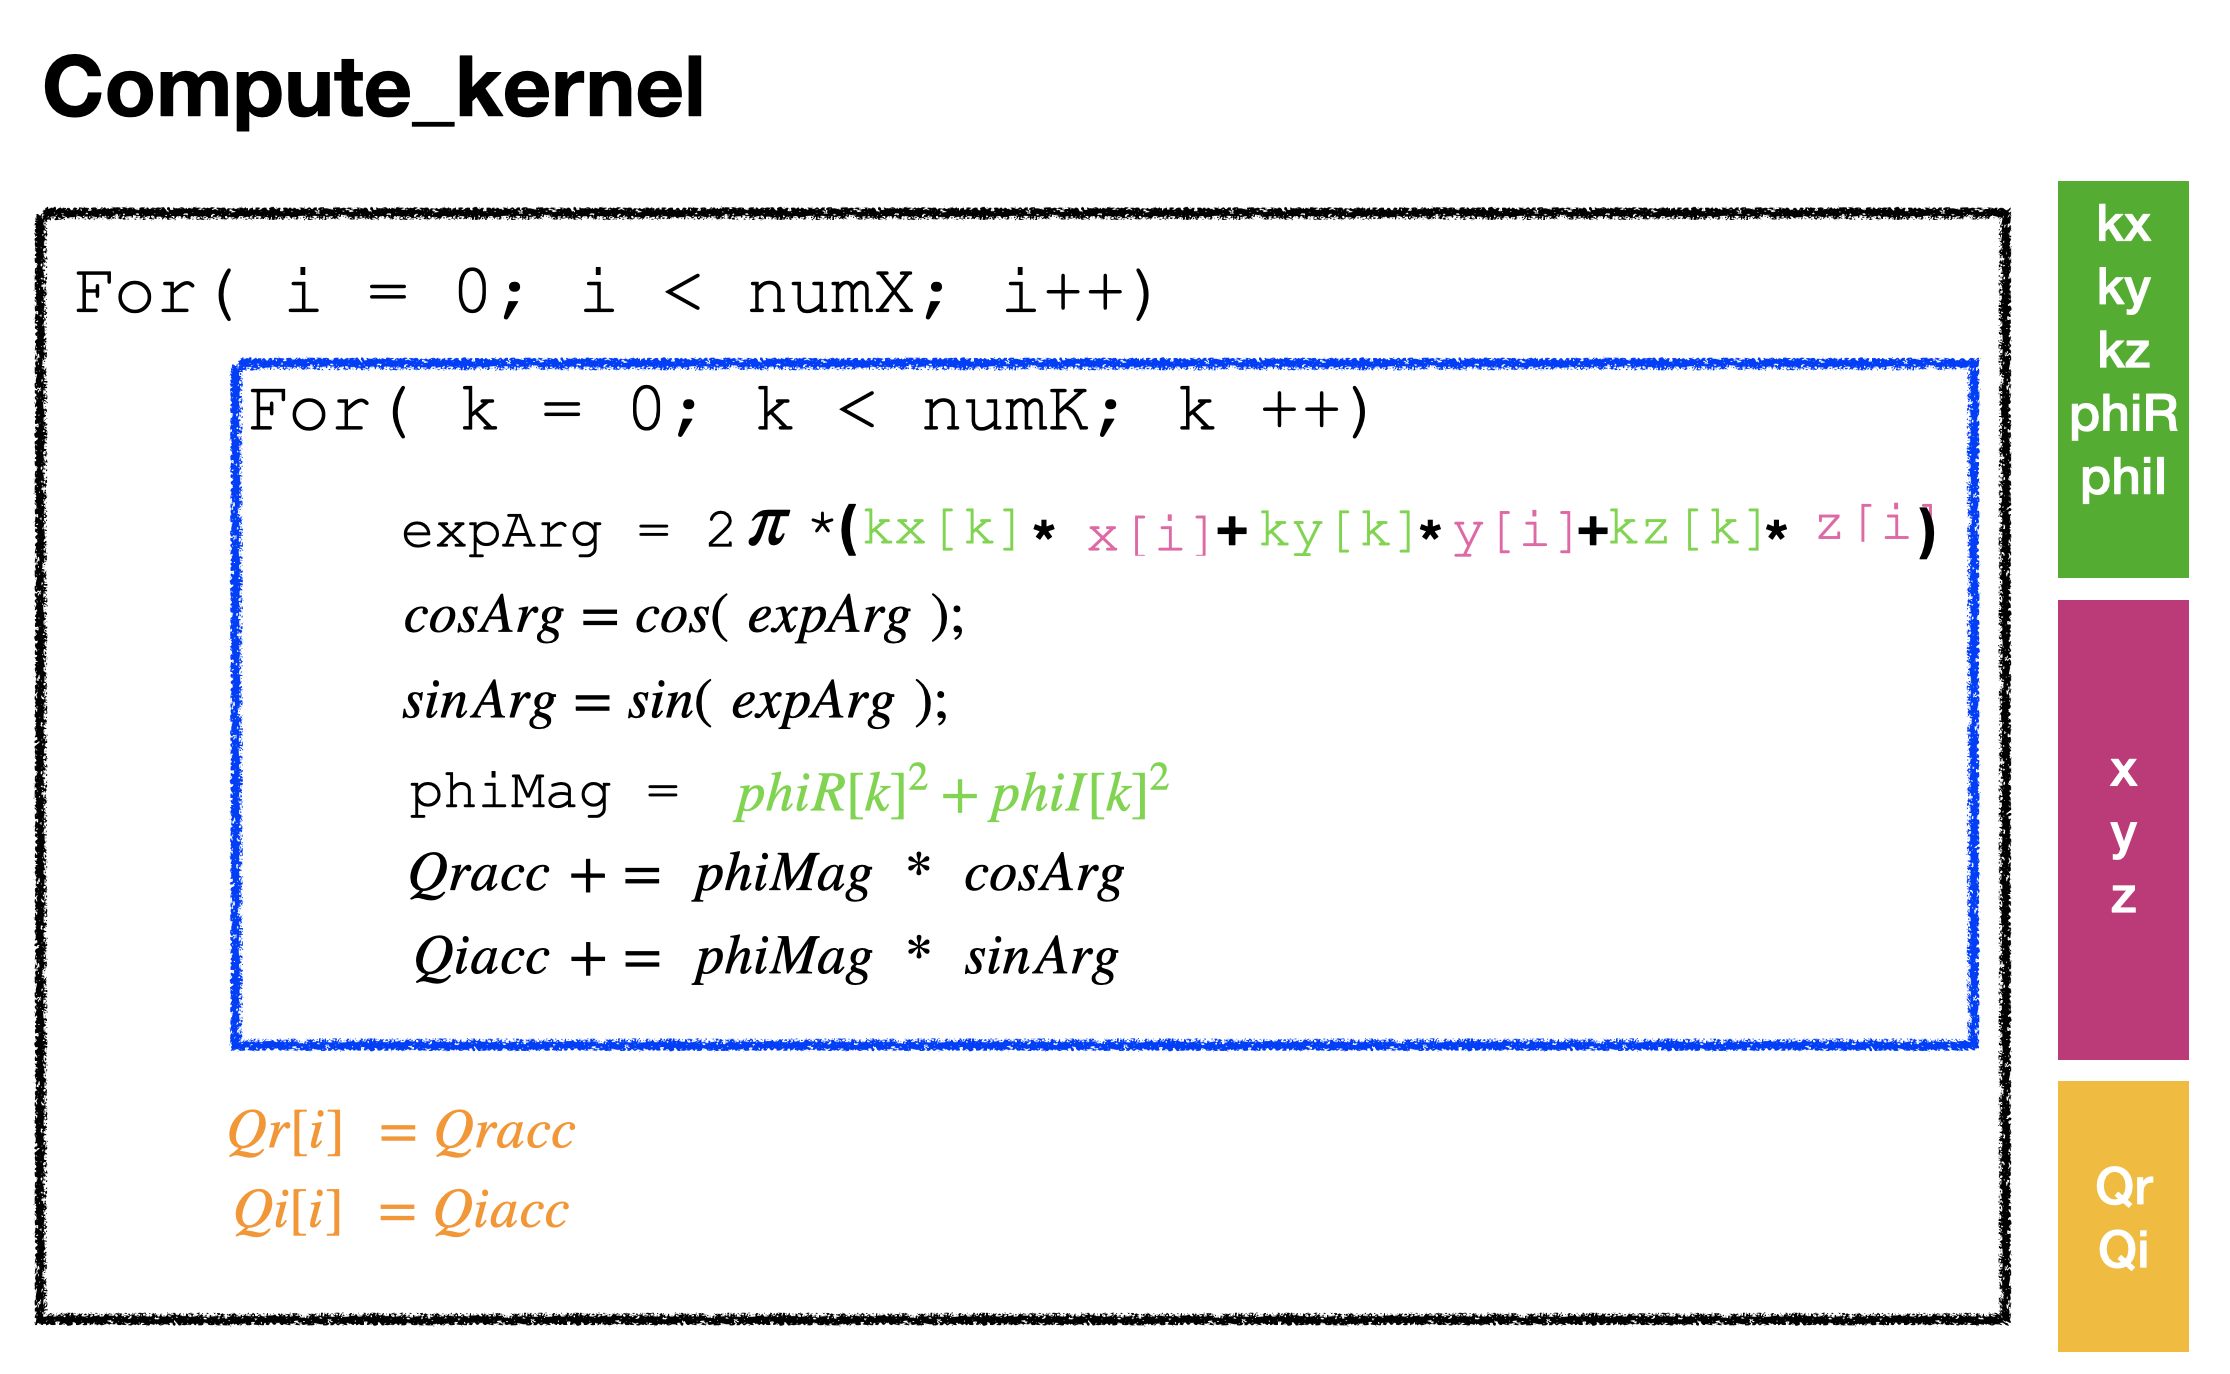
\includegraphics[width=0.85\columnwidth]{figure/algorithm.png}
\caption{Algorithm for computing MRI Q matrix~\cite{stone2008accelerating}}
\label{fig-1}
\end{figure}


\vspace{-4mm}
\section{Progress}

\subsection{Programmer View Implementation}
The Parboil benchmark provides datasets to run the programmer view implementation, shown in Table \ref{tab-1}. For input data with image size "small" and "medium", the execution takes 4.7s and 18.7s running on the google server (socp03), respectively. But for the "large" dataset, the run time is 186685s $ \sim$ 2.2 days. The higher precision of the reconstructed image, the bigger the input data size, and the more computation.
\begin{table}[h!]
    \centering
    \begin{tabular}{c|c|c|c}
    \hline
       name  & image size & \# of pixels & K-space dimension  \\
    \hline
        small  & 32*32*32 & 32768 & 3072 \\
        medium & 64*64*64 & 262144 & 2048\\
        large & 128*128*128 & 2097152 & 2097152\\
        \hline
    \end{tabular}
    \caption{Datasets of MRIQ from Parboil Benchmark}
    \label{tab-1}
\end{table}
\subsection{Behavioral Simulation}
I generated skeleton code from the ESP template with two configurable registers: numX and numK, which corresponds to the \# of pixels and K-space dimemsion in Table \ref{tab-1}. Then I edited the code in the following files:\\
\vspace{-2mm}
\begin{itemize}[leftmargin=*]
\item \textbf{mriq/hw/src/fpdata.hpp}\\
    Add fpdata.hpp to src/ folder. Typedef FPDATA. Defined functions used to do datatype conversions, for example, int2fp(), fp2int(), fp2bv(), bv2fp(). These functions are used in both the testbench and different processes of the accelerator design. In the testbench, data in floating-point type read from files is converted to fto fixed-point representation, then converted to sc\_bv to be transported through the network-on-chip. In accelerator, data in sc\_bv  type is converted to sc\_int to be stored in PLM. In computation phase, sc\_int data is converted to fixed -point representation.. After computation finished, The fixed-point data needs to be converted back to sc\_int in order to be stored in PLM. Then, it is further converted to sc\_bv to be transported back to the testbench for validation. In testbench, sc\_bv is converted to fixed-point representation. and further converted to floating point type to be compared with the golden output data.
  \vspace{-2mm}
   %%%%%%%
    \item \textbf{mriq/hw/src/mriq.hpp}\\
    I declared 10 PLMs, with name plm\_x, plm\_y, plm\_z, plm\_kx, plm\_ky, plm\_kz,  plm\_phiR, plm\_phiI, plm\_Qr,  plm\_Qi, and declared functions \textit{mySinf}, \textit{computeQ}, \textit{load\_one\_data}, and \textit{store\_one\_data}, used in mriq.cpp.
    \vspace{-2mm}
  %%%%%%%%%%%%%%%%%%%%%
    \item \textbf{mriq/hw/src/mriq.cpp}\\
Rewrote the processes \textit{load\_input},\textit{compute\_kernel}, \\
and  \textit{store\_output}. 
    \vspace{-2mm}
\item \textbf{mriq/hw/src/mriq\_functions.hpp}\\
    Wrote function \textit{ComputeQ} which is the key computation part of Q matrix, showed in Fig.\ref{fig-1}. Wrote function \textit{mySinf}, which is to compute sine. In sine function, first convert an input value to $0\sim \pi/2$ range, then find the closest data point in the sin\_table. For now, I use the interpolation method to get the sin(x). \textit{load\_one\_data} function is to load one variable into one PLM. Similarly, \textit{store\_one\_data} is to store one variable into one PLM.
    \vspace{-2mm}
    %%%%%%%%%%%%%%%%%%%%%%%%%%%%%%
    \item \textbf{mriq/hw/tb/system.hpp}\\
    Declared the paths for input file and golden output file. Modified the SC\_HAS\_PROCESS constructor. Declared parameters and functions used in system.cpp file.
        \vspace{-2mm}
    \item \textbf{mriq/hw/tb/system.cpp}\\
    Rewrote functions \textbf{\textit{load\_memory}}, \textbf{\textit{dump\_memory}}, and \textbf{\textit{validate}}. Added function \textbf{\textit{inputData}} to read input data from file, and \textbf{\textit{outputData}} to read golden output data from file.
        \vspace{-2mm}
    \item \textbf{mriq/hw/tb/sc\_main.cpp}\\
    Added the paths and names of the input file and the golden output file.
\end{itemize}
Behavioral simulation succeeded when running the whole dataset (32*32*32). It takes a few hours to run since the fixed-point datatype is not native to c/c++. 

\subsection{RTL generation}
I have generated RTL successfully by running make mriq-hls in the working folder. In this process, all the print sentences in the files in the src/ folder should be deleted to avoid that the ESP\_REPORT causes errors in this process. In every for-loop, there should be a wait() sentence after the "for statement" to allow Stratus to perform loop unrolling.

\subsection{RTL Simulation}
By running an accelerated simulation method, I have tested the generated RTL without error. Instead of computing the whole dataset, which has 32K pixels, I edited the code to compute only the first 4 pixels in the input dataset and reduced the k-space size from 3K to 16. The simulation of RTL succeeded. My accelerating method of simulation is to edit the default value of (numX, numK) from (32768, 3072) to (4, 16) both in tb/system.hpp and src/mriq\_conf\_info.hpp. 

\section{Future Work}

\subsection{Accelerator Integration}
Finish the accelerator integration and prototpye on FPGA.

\subsection{Design Space Exploration}
There are two directions for design space exploration. The first is to reduce latency. The optimization methods I plan to do is as follows:
\begin{enumerate}
\setlength\itemsep{-0.15em}
\item Loop unroll and pipeline.
\item Constrain latency.
\item Reduce fixed-point precision.
\item Add more ports to PLM to increase parallelism.
\item Optimize compute function. Optimize the computation of sine and cosine functions.
\end{enumerate}
The second direction is to reduce area. The following are the methods I plan to try.
\begin{enumerate}
\setlength\itemsep{-0.15em}
    \item Use ping pong buffers to load a portion of data to do computation. Load all the frequency-related variables (kx, ky, kz, phiR, phiZ) into PLM, but only load a portion of pixels (x,y,z). 
    \item In place storage of output. 
    \item Use different types of PLM blocks. frequency-related variables are stored in one type of PLM with size numK. The pixel variables (x,y,z) could be stored in a much smaller PLM block if using ping-pong buffers. 
    \item Reduce sine look-up table.  
    \item Reduce fixed-point storage. For now, data size is 32 bits. Later, I will try to reduce this data width while guaranteeing the computation accuracy. A smaller number of bits requires smaller storage capacity.
\end{enumerate}

I will generate a Pareto curve of my designs. Then, I will compare the FPGA running time with the software running time on FPGA to evaluate the performance of the accelerator.

%Bibliography
{\small
\balance
%\bibliographystyle{abbrv}
\bibliographystyle{unsrt}
\bibliography{ref}
}


% If you need to add an appendix with large figures or table use the following
% code:

%% \newpage
%% \onecolumn{
%% \centering
%% \section*{APPENDIX}
%% \vspace{0.5in}

%% % Add your Appendix text and figures here.

%% }

\end{document}
